\documentclass[12pt, a4paper]{article}
\usepackage[utf8]{inputenc}
\usepackage[italian]{babel}
\usepackage[T1]{fontenc}
\usepackage{geometry}
\usepackage{booktabs}
\usepackage{hyperref}
\usepackage{parskip}
\usepackage{array}
\usepackage{float}
\usepackage{graphicx}
 
\geometry{margin=2.5cm}
 
\title{\textbf{Abbandono lavorativo: analisi e previsioni sul dataset}\\ 
\large Progetto di fine corso }
\author{\textbf{Gruppo 5} \\ Isabella Manetti \\ Elisa Mezzi \\ Maddalena Vannini }
\date{Appello 8 Luglio 2026}
 
\begin{document}
 
\maketitle
 
% -------------------------------------------------------
\section{Introduzione}
 
Il presente report, che costituisce il progetto finale del corso di \textit{Introduzione alla Data Science e al pensiero computazionale}, ha come obiettivo la costruzione di un modello che stimi la probabilità che un dipendente lasci l'azienda sulla base di caratteristiche demografiche, lavorative ed economiche. 
La variabile target è \texttt{Attrition} (dove la classe \textit{Yes} indica chi abbandona il lavoro, mentre la classe \textit{No} chi non lo abbandona). 
 
L'abbandono dei dipendenti -- noto in letteratura anglosassone come \textit{employee attrition} -- indica la riduzione graduale del personale dovuta all'uscita di dipendenti dall'organizzazione, per ragioni volontarie o involontarie, senza che le posizioni vengano necessariamente sostituite \cite{aihr2026}. Si tratta di un indicatore critico per le organizzazioni, poiché influenza direttamente la produttività, il clima aziendale e i costi di gestione delle risorse umane.

Il report è diviso in tre fasi: la prima è dedicata alla descrizione del Dataset e a una prima analisi di dati; nella seconda fase verranno messe in relazione diverse feature con un focus sulla variabile \texttt{Attrition}; la terza e ultima fase si concentra sulla costruzione di tre modelli predittivi: k-NN, Random Forest e regressione logistica, basata sulla relazione tra le variabili \texttt{Attrition} e \texttt{MonthlyIncome}.

Come vedremo nei prossimi paragrafi, il problema principale del report analizzato è lo sbilanciamento tra le due classi della variabile \texttt{Attrition} (Yes/No), essendo la classe \textit{No} nettamente predominante. Ciò influisce negativamente sulla robustezza di tutti i modelli elaborati: mentre l'accuracy risulta molto elevata, dal momento che i modelli predicono correttamente chi non abbandona il lavoro, la matrice di confusione e gli altri valori analizzati (precision, recall e f1-score) mostrano i tre modelli in tutta la loro fragilità.
 
% -------------------------------------------------------
\section{Fase 1: descrizione e comprensione del dataset }
\textit{di Maddalena Vannini}

\subsection{Descrizione del Dataset e prima EDA}

Questa prima fase è dedicata alla comprensione della struttura del dataset e all'analisi preliminare dei dati, propedeutica alle fasi successive di modellazione.
Il dataset è composto da \textbf{1.470 righe} (una per dipendente) e \textbf{35 colonne} (variabili). Non sono stati rilevati valori mancanti (\textit{null}) in nessuna delle colonne.
 
Le variabili sono state classificate in tre categorie:
 
\begin{itemize}
    \item \textbf{Variabili numeriche continue} (chiamate \texttt{Numeriche}): valori quantitativi come età, reddito mensile, anni in azienda (es. \texttt{Age}, \texttt{MonthlyIncome}, \texttt{YearsAtCompany}).
    \item \textbf{Variabili categoriche nominali} (chiamate \texttt{Categoriche pure}): valori testuali senza ordine intrinseco, come \texttt{Department}, \texttt{Gender}, \texttt{MaritalStatus}, \texttt{OverTime}.
    \item \textbf{Variabili categoriche ordinali} (chiamate \texttt{Categoriche codificate}): valori numerici che rappresentano livelli ordinati con un significato qualitativo, come \texttt{JobSatisfaction} (1=Low, 4=Very High) ed \texttt{Education} (1=Below College, 5=Doctor).
\end{itemize}
 
Sono state identificate tre colonne non informative, in quanto costanti per tutti i dipendenti: \texttt{EmployeeCount} (sempre 1), \texttt{StandardHours} (sempre 80) e \texttt{Over18} (sempre ``Y''), pertanto queste variabili non sono state prese in considerazione nelle analisi successive.
 
% -------------------------------------------------------

\subsection{Statistiche descrittive delle variabili numeriche e categoriche}

I dipendenti osservati hanno età compresa tra 18 e 60 anni (media 37 anni); il reddito mensile presenta una distribuzione fortemente asimmetrica: pur registrando una media di 6.503\$, la mediana si attesta 
a 4.919\$, a indicare che la metà dei dipendenti guadagna al di sotto di tale soglia e che alcuni stipendi molto elevati alzano la media.

Tra le variabili categoriche, quasi il 30\% dei dipendenti dichiara di svolgere straordinari; il reparto più rappresentato è R\&D con il 65\% dei dipendenti, mentre HR conta solo il 4.3\%. Il 71\% dei dipendenti viaggia raramente per lavoro, il 18.8\% frequentemente e il restante 10\% non viaggia affatto. Sul fronte della formazione, il titolo di studio più diffuso è il Bachelor (38.9\%), seguito dal 
Master (27.1\%); i Doctor rappresentano la minoranza(3.3\%).

Le variabili ordinali mostrano distribuzioni concentrate sui valori medio-alti della scala. Il 59\% dei dipendenti dichiara un coinvolgimento lavorativo ``High'' (\texttt{JobInvolvement = 3}), e il 60.7\% valuta il proprio equilibrio casa-lavoro come migliore della media (\texttt{WorkLifeBalance = 3}). 
Solo il 5.4\% riporta un equilibrio ``Bad''.

Da menzionare la variabile \texttt{PerformanceRating} che presenta un'anomalia rilevante: 
nel dataset compaiono esclusivamente i valori 3 (Excellent) e 4 (Outstanding), con \textit{totale assenza dei livelli 1 e 2}. Una possibile spiegazione è che i dipendenti con performance bassa siano stati 
rimossi dal dataset prima della raccolta, introducendo un potenziale 
\textit{bias di selezione} che andrà tenuto in considerazione nelle fasi successive. 

\subsection{Distribuzione della variabile target}
 
In questo campione, la variabile target \texttt{Attrition} presenta una distribuzione sbilanciata: l'\textbf{83.9\%} dei dipendenti è rimasto in azienda (\texttt{No}), mentre solo il \textbf{16.1\%} ha lasciato (\texttt{Yes}), cioè 237 dipendenti su 1.470. Questo squilibrio dovrà essere gestito nella fase di modellazione.
 
Per orientare le fasi successive, è stata condotta un'\textbf{analisi bivariata elementare} tra \texttt{Attrition} e alcune variabili di interesse prese in considerazione per formulare le prime ipotesi.
 
\begin{table}[H]
\centering
\begin{tabular}{lcc}
\toprule
\textbf{Variabile} & \textbf{Attrition = No} & \textbf{Attrition = Yes} \\
\midrule
\multicolumn{3}{l}{\textit{JobSatisfaction}} \\
\midrule
1 (Low) & 77.2\% & 22.8\% \\
2 (Medium) & 83.6\% & 16.4\% \\
3 (High) & 83.5\% & 16.5\% \\
4 (Very High) & 88.7\% & 11.3\% \\
\midrule
\multicolumn{3}{l}{\textit{OverTime}} \\
\midrule
No & 89.6\% & 10.4\% \\
Yes & 69.5\% & 30.5\% \\
\midrule
\multicolumn{3}{l}{\textit{BusinessTravel}} \\
\midrule
Non-Travel & 92.0\% & 8.0\% \\
Travel\_Rarely & 85.0\% & 15.0\% \\
Travel\_Frequently & 75.1\% & 24.9\% \\
\midrule
\multicolumn{3}{l}{\textit{Department}} \\
\midrule
Human Resources & 80.9\% & 19.1\% \\
Research \& Development & 86.2\% & 13.8\% \\
Sales & 79.4\% & 20.6\% \\
\bottomrule
\end{tabular}
\caption{Distribuzione percentuale di Attrition per variabili categoriche.}
\end{table}

\begin{table}[H]
\centering
\begin{tabular}{lcc}
\toprule
\textbf{Variabile} & \textbf{Attrition = No} & \textbf{Attrition = Yes} \\
\midrule
MonthlyIncome (\$) & 6.833 & 4.787 \\
Age (anni) & 37.6 & 33.6 \\
NumCompaniesWorked & 2.6 & 2.9 \\
YearsSinceLastPromotion & 2.2 & 1.9 \\
\bottomrule
\end{tabular}
\caption{Confronto delle medie tra dipendenti rimasti e usciti per variabili numeriche.}
\end{table}
 
Le associazioni più marcate con \texttt{Attrition} riguardano lo svolgimento di straordinari e la frequenza dei viaggi di lavoro; per le variabili numeriche, si osserva che i dipendenti usciti dall'azienda avevano in media un reddito mensile e un'età inferiori rispetto a chi è rimasto, mentre il numero di aziende precedenti e gli anni dall'ultima promozione mostrano differenze contenute, non sufficienti a suggerire un'associazione forte.
% -------------------------------------------------------
\subsection{Osservazioni Critiche}
 
\begin{itemize}
    \item \textbf{Class imbalance}: il dataset è fortemente sbilanciato verso il valore \texttt{Attrition = No}. Ciò potrebbe portare il modello a predire sempre ``No'', ottenendo un'accuratezza alta ma non significativa.
 
    \item \textbf{Feature sospette}: la variabile \texttt{PerformanceRating} presenta esclusivamente i valori 3 (Excellent) e 4 (Outstanding), con totale assenza dei valori 1 e 2. È probabile che i dipendenti con performance bassa siano stati rimossi dal dataset prima della raccolta, introducendo un \textit{bias di selezione}.

\end{itemize}
 
% -------------------------------------------------------
\subsection{Conclusioni}
 
Il dataset si presenta pulito e privo di valori mancanti, ma con alcune criticità rilevanti: il forte sbilanciamento della variabile target, la presenza di variabili costanti da eliminare e un possibile pre-filtraggio dei dati relativo alla performance. Le analisi preliminari suggeriscono che le variabili \texttt{OverTime}, \texttt{MonthlyIncome} e \texttt{BusinessTravel} abbiano le associazioni più marcate con l'abbandono e meritino attenzione nelle fasi successive.


\subsection*{Nota sull'uso dell'IA}
Per lo sviluppo di questa prima parte, è stato usato l’LLM Claude come assistente AI, innanzitutto per correggere errori di codice in fase di esplorazione dei dati, poi per alcune task specifiche come in fase di setting del notebook, per collegare correttamente il dataset da GitHub in Colab via URL raw; in fase EDA per avere chiarimenti sulle descrizioni delle variabili del dataset, per cercare possibili motivazioni per cui la variabile PerformanceRating è incompleta e se queste fossero rilevanti, e infine come aiuto per la revisione di questa sezione del paper (es. stilizzazione tabella paragrafo 2.3).

\section{Fase 2: analisi esplorativa e visualizzazione}
\textit{di Elisa Mezzi}

L'analisi esplorativa è stata svolta con la libreria \texttt{seaborn} ed è impostata nel seguente modo: con le heatmap si parte dallo studio delle correlazioni per capire quali variabili sono associate
all'abbandono (\texttt{Attrition}) e quali sono ridondanti tra loro, per poi approfondire con grafici
dedicati alle singole variabili. La correlazione è misurata con il coefficiente di Pearson, definito tra due
variabili $x$ e $y$ come:
\begin{equation}
r_{xy} = \frac{\sum_{i=1}^{n}(x_i - \bar{x})(y_i - \bar{y})}
{\sqrt{\sum_{i=1}^{n}(x_i - \bar{x})^2}\,\sqrt{\sum_{i=1}^{n}(y_i - \bar{y})^2}}
\end{equation}
con valori in $[-1,+1]$: il segno indica la direzione della relazione, il valore assoluto la sua
forza. Le variabili categoriche sono state codificate in variabili indicatrici (0/1) e la target in
forma binaria (\texttt{Attrition\_bin}) per poterle includere nell'analisi di correlazione \cite{slide}.

\subsection{La distribuzione della variabile target}
Il primo passo è osservare la distribuzione di \texttt{Attrition} (Figura~\ref{fig:target}). Il dataset
è fortemente \textbf{sbilanciato}: 1233 dipendenti (83,9\%) sono rimasti e solo 237 (16,1\%) hanno
abbandonato. Questo squilibrio guiderà tutto il resto dell'analisi.
\begin{figure}[H]
\centering
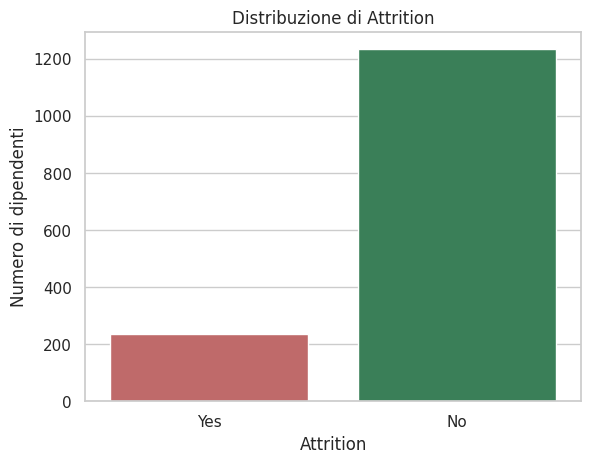
\includegraphics[width=0.5\textwidth]{Images/distr_attrition.png}
\caption{Distribuzione della variabile target \texttt{Attrition}.}
\label{fig:target}
\end{figure}

\subsection{Le relazioni significative con l'abbandono}
Lo studio prosegue con due heatmap di correlazione, lette innanzitutto
lungo la riga della variabile target per individuare le variabili più legate all'abbandono.
\begin{figure}[H]
\centering
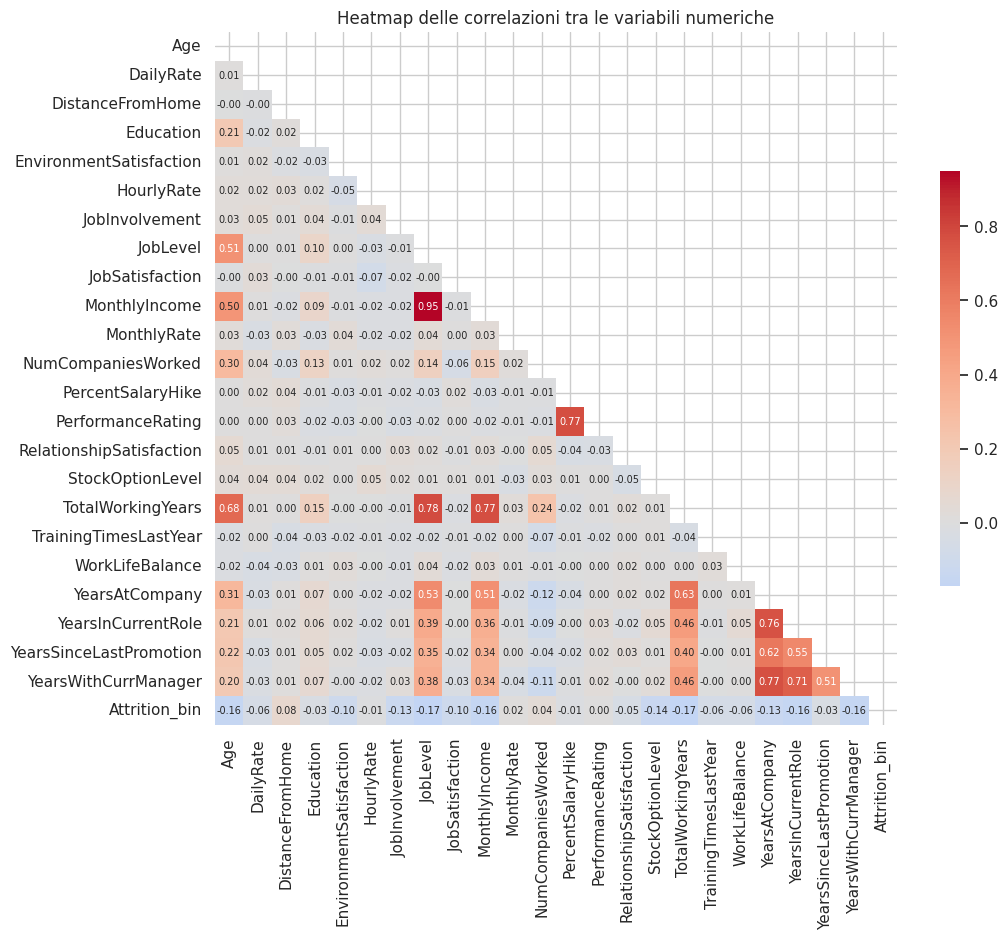
\includegraphics[width=0.7\textwidth]{Images/heatmap_numeriche.png}
\caption{Heatmap di correlazione tra le variabili numeriche.}
\label{fig:hnum}
\end{figure}
\textbf{Variabili numeriche.} Le più correlate con l'abbandono presentano tutte una relazione
\emph{negativa}: \texttt{TotalWorkingYears}, \texttt{JobLevel}, \texttt{MonthlyIncome} e \texttt{Age}
(intorno a $-0{,}17$), seguite da \texttt{StockOptionLevel} ($-0{,}14$), \texttt{JobInvolvement}
($-0{,}13$) e dalle variabili di anzianità (\texttt{YearsAtCompany}, \texttt{YearsInCurrentRole}, \texttt{YearsWithCurrManager}, \texttt{YearsSinceLastPromotion}). All'aumentare di esperienza, livello, reddito, età e
coinvolgimento, l'abbandono diminuisce. Anche \texttt{JobSatisfaction} ed
\texttt{EnvironmentSatisfaction} mostrano una relazione negativa più contenuta.
L'unica leggermente \emph{positiva} è \texttt{DistanceFromHome} ($+0{,}08$), mentre
\texttt{MonthlyRate}, \texttt{HourlyRate} e \texttt{PercentSalaryHike} hanno correlazione quasi nulla.
\begin{figure}[H]
\centering
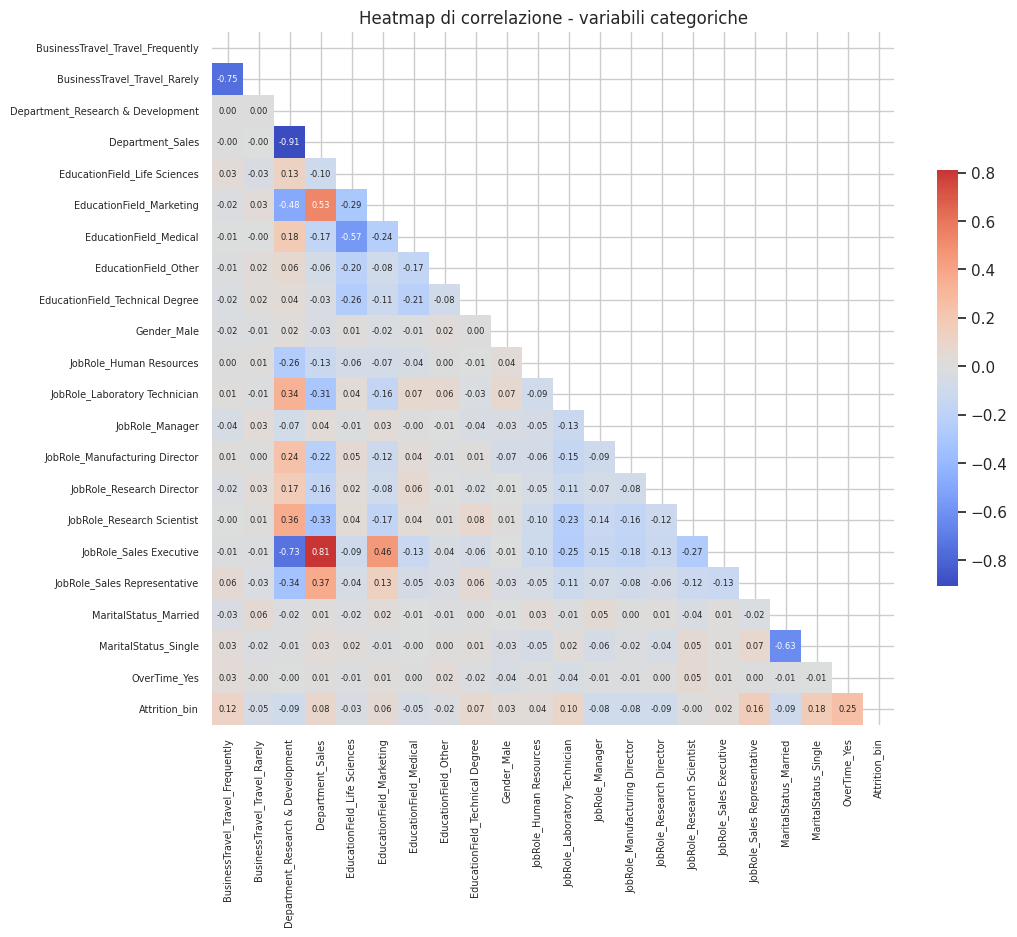
\includegraphics[width=0.7\textwidth]{Images/heatmap_categoriche.png}
\caption{Heatmap di correlazione tra le variabili categoriche.}
\label{fig:hcat}
\end{figure}
\textbf{Variabili categoriche.} Le categorie più associate all'abbandono sono \texttt{OverTime\_Yes}
($+0{,}25$, la più alta del dataset), \texttt{MaritalStatus\_Single} ($+0{,}18$),
\texttt{JobRole\_Sales Representative} ($+0{,}16$) e \texttt{BusinessTravel\_Travel\_Frequently}
($+0{,}12$). Hanno invece relazione negativa \texttt{MaritalStatus\_Married},
\texttt{Department\_Research \& Development} e i ruoli direttivi.

\subsection{Caratteristiche personali del dipendente}
Sono state poi analizzate le caratteristiche anagrafiche (Figura~\ref{fig:personali}). L'\textbf{età}
ha un effetto netto: i più giovani abbandonano molto di più (nella fascia 18--25 anni il 35,8\%), e il tasso scende progressivamente fino a circa il 9\% nelle fasce 36--45.
Il \textbf{genere}, invece, incide poco: gli uomini abbandonano il 17,0\% e le donne il 14,8\%, una
differenza minima coerente con la correlazione quasi nulla vista nella heatmap. Lo \textbf{stato
civile} è invece molto rilevante: i single abbandonano il 25,5\%, contro il 12,5\% dei coniugati e il
10,1\% dei divorziati.
\begin{figure}[H]
\centering
\begin{minipage}{0.32\textwidth}\centering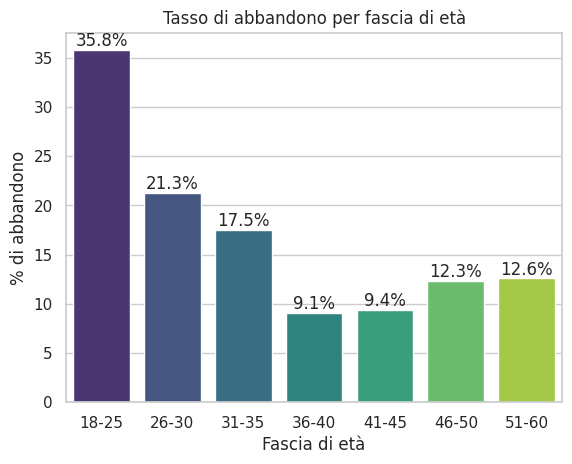
\includegraphics[width=\linewidth]{Images/Età_attrition.png}\end{minipage}\hfill
\begin{minipage}{0.32\textwidth}\centering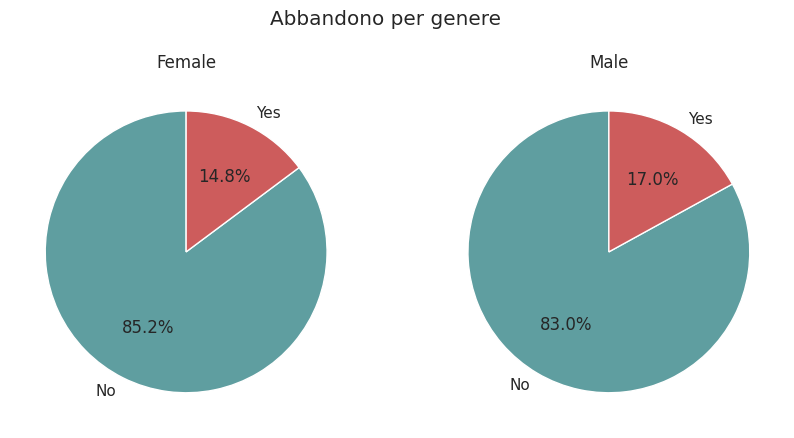
\includegraphics[width=\linewidth]{Images/Genere_Attrition.png}\end{minipage}\hfill
\begin{minipage}{0.32\textwidth}\centering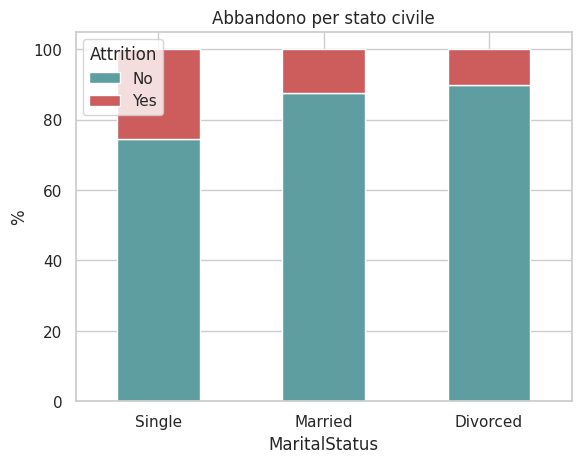
\includegraphics[width=\linewidth]{Images/MaritalStatus_Attrition.png}\end{minipage}
\caption{Caratteristiche personali: tasso di abbandono per fascia di età, per genere e per stato civile.}
\label{fig:personali}
\end{figure}

\subsection{Condizioni di lavoro e coinvolgimento}
Due variabili risultano tra le più informative (Figura~\ref{fig:lavoro}). Gli \textbf{straordinari}
sono il segnale più forte in assoluto: chi fa \texttt{OverTime} abbandona il 30,5\%, contro il 10,4\%
di chi non li fa, quasi tre volte tanto. Il \textbf{coinvolgimento nel lavoro}
(\texttt{JobInvolvement}) mostra un andamento decrescente molto regolare: il tasso di abbandono passa
dal 33,7\% del livello più basso al 9,0\% del più alto, segno di una relazione chiara.
\begin{figure}[H]
\centering
\begin{minipage}{0.49\textwidth}\centering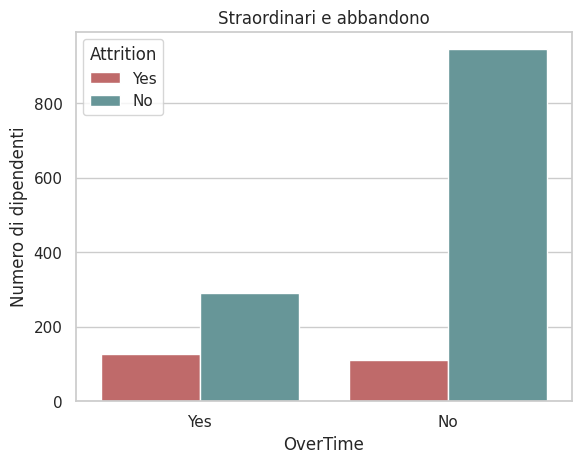
\includegraphics[width=\linewidth]{Images/OverTime_Attrition.png}\end{minipage}\hfill
\begin{minipage}{0.49\textwidth}\centering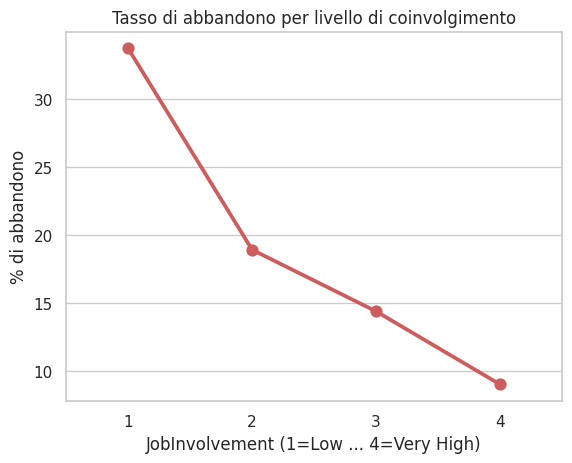
\includegraphics[width=\linewidth]{Images/JobInvolvement_Attrition.png}\end{minipage}
\caption{Condizioni di lavoro: abbandono per \texttt{OverTime} e per livello di \texttt{JobInvolvement}.}
\label{fig:lavoro}
\end{figure}

\subsection{Variabili economiche}
Per quanto riguarda gli aspetti retributivi (Figura~\ref{fig:economia}), il \textbf{reddito mensile} (\texttt{MonthlyIncome})
distingue bene i due gruppi: chi abbandona ha una mediana sensibilmente più bassa (circa 3200\$ contro
5200\$). Al contrario, il \textbf{MonthlyRate} non mostra alcuna differenza tra chi resta e chi
abbandona. Le
\textbf{stock option} (\texttt{StockOptionLevel}) confermano l'idea che gli incentivi economici
trattengano: chi non ne ha (livello 0) abbandona di più rispetto ai livelli 1 e 2;
fa eccezione il livello 3, dove l'abbandono risale, ma il gruppo è poco numeroso e va letto con
cautela.
\begin{figure}[H]
\centering
\begin{minipage}{0.32\textwidth}\centering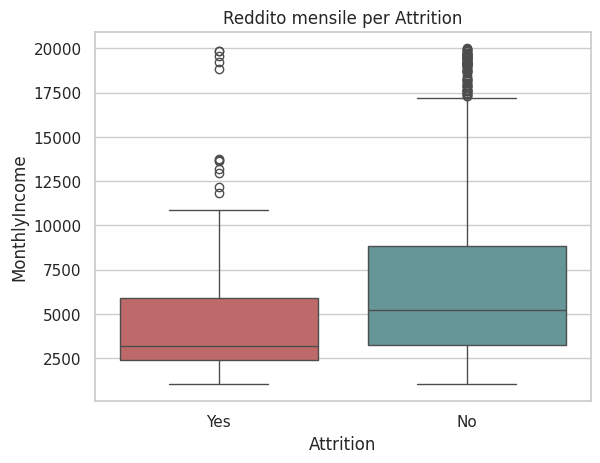
\includegraphics[width=\linewidth]{Images/MonthlyIncome_Attrition.png}\end{minipage}\hfill
\begin{minipage}{0.32\textwidth}\centering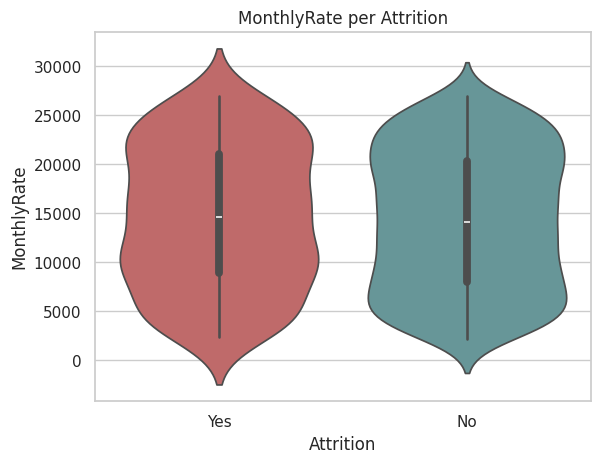
\includegraphics[width=\linewidth]{Images/MonthlyRate_Attrition.png}\end{minipage}\hfill
\begin{minipage}{0.32\textwidth}\centering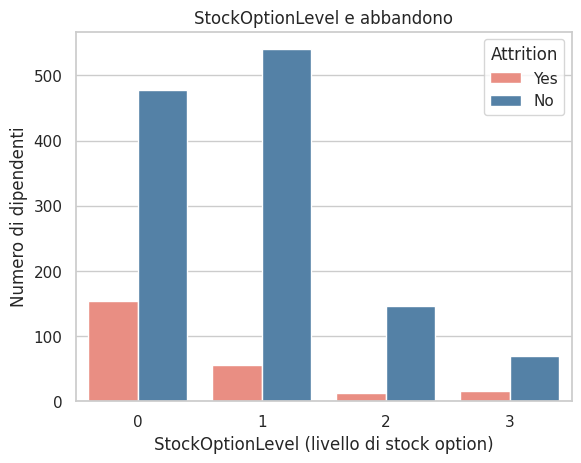
\includegraphics[width=\linewidth]{Images/StockOptionLevel_Attrition.png}\end{minipage}
\caption{Variabili economiche: reddito mensile, MonthlyRate e livello di stock option.}
\label{fig:economia}
\end{figure}

\subsection{Ruolo e anzianità}
Il \textbf{ruolo} (\texttt{JobRole}) è una delle variabili più discriminanti (Figura~\ref{fig:ruolo}):
si passa dal 39,8\% di abbandono dei \emph{Sales Representative} al 2,5\% dei \emph{Research Director}.
L'\textbf{anzianità in azienda} (\texttt{YearsAtCompany}) mostra che chi abbandona è in azienda da meno
tempo: gli abbandoni si concentrano nei primi anni e diventano rari con il crescere dell'anzianità.
\begin{figure}[H]
\centering
\begin{minipage}{0.55\textwidth}\centering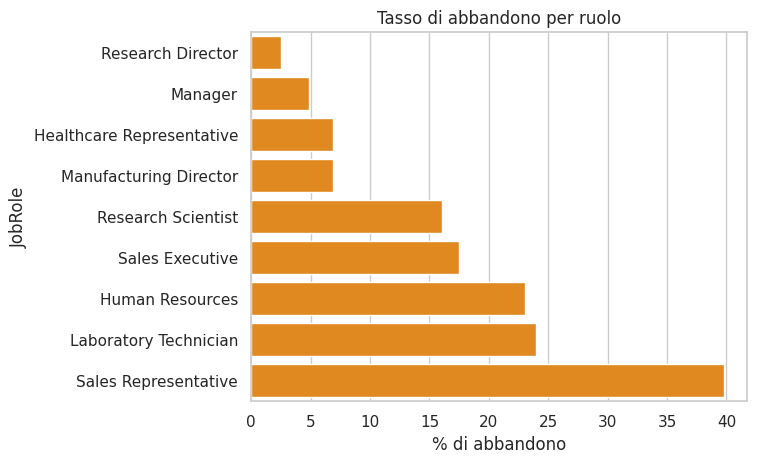
\includegraphics[width=\linewidth]{Images/JobRole_Attrition.png}\end{minipage}\hfill
\begin{minipage}{0.43\textwidth}\centering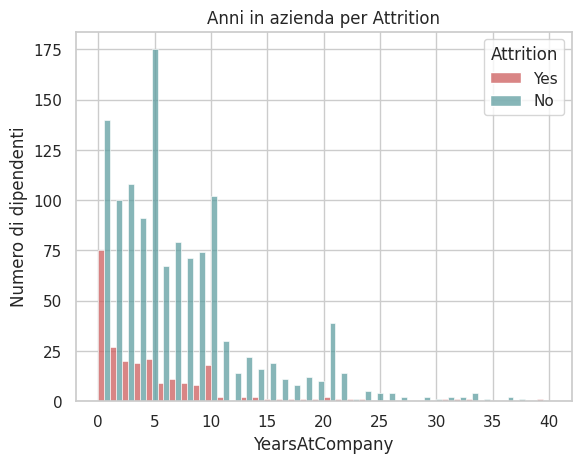
\includegraphics[width=\linewidth]{Images/YearsAtCompany_Attrition.png}\end{minipage}
\caption{Ruolo e anzianità: tasso di abbandono per \texttt{JobRole} e distribuzione di
\texttt{YearsAtCompany} per classe.}
\label{fig:ruolo}
\end{figure}

\subsection{Confronti tra variabili}
Infine, le forti correlazioni tra variabili emerse nelle heatmap sono state verificate
visivamente con dei confronti diretti (Figura~\ref{fig:confronti}). \texttt{JobLevel} e
\texttt{MonthlyIncome} crescono quasi insieme ($r=0{,}95$): il reddito aumenta in modo regolare con il
livello di carriera, quindi le due variabili sono ridondanti. Lo stesso vale, in misura più contenuta,
per \texttt{Age} e \texttt{TotalWorkingYears} ($r=0{,}68$). Al contrario,
\texttt{NumCompaniesWorked} e \texttt{YearsAtCompany} hanno una relazione \emph{negativa} e debole
($r\approx-0{,}12$): chi ha cambiato più aziende ha meno anni di permanenza nell'attuale, ma il legame
è quasi assente, quindi le due variabili sono sostanzialmente indipendenti.
\begin{figure}[H]
\centering
\begin{minipage}{0.32\textwidth}\centering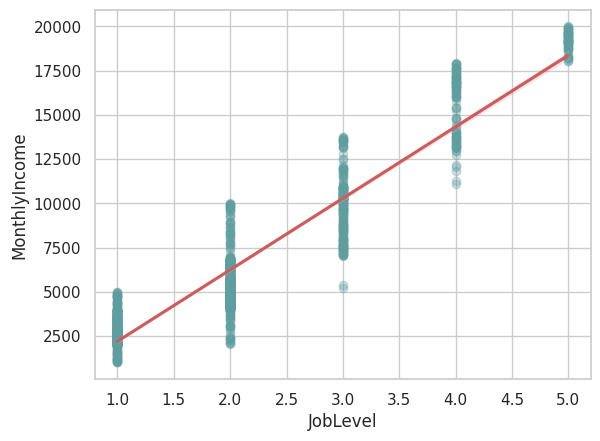
\includegraphics[width=\linewidth]{Images/MonthlyIncome_JobLevel_Attrition.png}\end{minipage}\hfill
\begin{minipage}{0.32\textwidth}\centering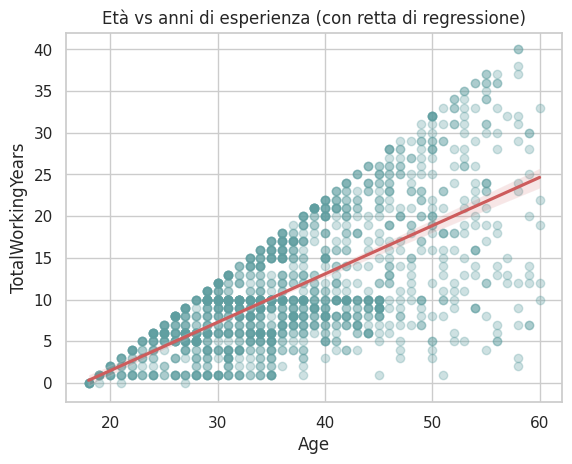
\includegraphics[width=\linewidth]{Images/TotalWorkingYears_Age.png}\end{minipage}\hfill
\begin{minipage}{0.32\textwidth}\centering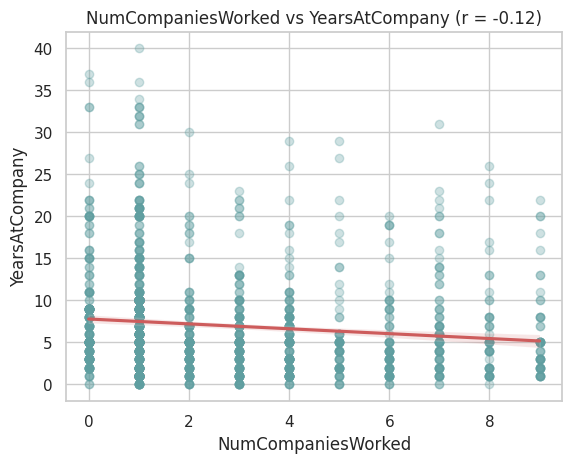
\includegraphics[width=\linewidth]{Images/YearsAtCompany_NumCompaniesWorked.png}\end{minipage}
\caption{Confronti tra coppie di variabili.}
\label{fig:confronti}
\end{figure}

\subsection{Osservazioni dell'analisi visiva ed esplorativa.}
L'analisi esplorativa permette di indicare quali variabili sono più \textbf{utili} a prevedere
l'abbandono: \texttt{OverTime}, \texttt{MaritalStatus}, \texttt{JobRole}, \texttt{BusinessTravel},
\texttt{JobInvolvement}, \\\texttt{StockOptionLevel}, \texttt{MonthlyIncome} e \texttt{Age}, ossia quelle
che mostrano le differenze più nette tra chi resta e chi se ne va. Alcune di queste, però, sono
fortemente correlate \textbf{tra loro} e risultano quindi \textbf{ridondanti}: in particolare
\texttt{JobLevel} e \texttt{MonthlyIncome}, le variabili di anzianità (\texttt{YearsAtCompany},
\texttt{YearsInCurrentRole}, \texttt{YearsWithCurrManager}) e la coppia \texttt{Age}--\texttt{TotalWorkingYears}.
Risultano invece \textbf{poco o per nulla informative} \texttt{MonthlyRate}, \texttt{HourlyRate},
\texttt{DailyRate}, \texttt{PercentSalaryHike} e \texttt{Gender}, mentre erano già state
\textbf{escluse a priori} le variabili costanti o identificative (\texttt{Over18},
\texttt{EmployeeCount}, \texttt{StandardHours}, \texttt{EmployeeNumber}) e \texttt{PerformanceRating},
perché incompleta. Va infine ricordato che le correlazioni osservate non implicano un rapporto di
causa-effetto: una relazione può sempre dipendere da una terza variabile non osservata.


\section{Fase 3: modellazione}
\textit{di Isabella Manetti}

In questa fase vengono costruiti e analizzati tre modelli predittivi: k-NN, Random Forest e regressione logistica. 
\\Quest'ultima mette in relazione le due variabili \texttt{Attrition} e \texttt{MonthlyIncome}, una delle variabili che più incidono sull'abbandono lavorativo.

Preliminarmente sono state rimosse le variabili che costituivano un "rumore" per i tre modelli: \texttt{EmployeeCount} (vale sempre 1), \texttt{EmployeeNumber} (rappresenta il numero identificativo del dipendente), \texttt{Over18} (tutti i dipendenti hanno più di 18 anni), \texttt{StandardHours} (vale sempre 8) e \texttt{PerformanceRating} (presenta solo le classi 3 e 4, risultando una variabile incompleta).

In seguito le variabili categoriche sono state trasformate in numeriche e, infine, il dataset originale è stato diviso in train e test, mantenendo la proporzione 80/20\%.

I tre modelli analizzati presentano caratteristiche comuni, conseguenza dello sbilanciamento delle due classi della variabile \texttt{Attrition}, \textit{No} e \textit{Yes}, in favore di chi non abbandona l'azienda:
\begin{itemize}
    \item L'accuracy dei tre modelli risulta piuttosto alta (85,4\% per k-NN, 82,7\% per Random Forest e 84\% per regressione lineare), ma ciò dipende dal fatto che i modelli stessi riescano a prevedere la classe \textit{No}, essendo questa in netta maggioranza;
    \item Le tre matrici di confusione smentiscono quanto riportato dall'accuracy, dal momento che i modelli riescono a prevedere correttamente solo chi non lascia l'azienda e, al contrario, non riescono a prevedere correttamente chi lascia l'azienda;
    \item Precision, recall e f1-score confermano quanto riportato da accuracy e matrice di confusione: queste metriche di valutazione, se relative alla classe \textit{No} rappresentano modelli forti, se relative alla classe \textit{Yes}, mostrano i modelli in tutta la loro fragilità.
\end{itemize}

\begin{figure}[H]
\centering
\begin{minipage}{0.32\textwidth}\centering
\includegraphics[width=\linewidth]{Confusion_matrix_k-nn.png}\end{minipage}\hfill
\begin{minipage}{0.32\textwidth}\centering
\includegraphics[width=\linewidth]{Confusion_matrix_random_forest.png}\end{minipage}\hfill
\begin{minipage}{0.32\textwidth}\centering
\includegraphics[width=\linewidth]{Confusion_matrix_regressione_logistica.png}\end{minipage}
\caption{Matrici di confusione per k-NN, Random Forest e regressione logistica}
\label{fig:personali}
\end{figure}

I risultati dell'analisi vengono confermati dall'osservazione sull'accuracy su più livelli di k, per il modello k-NN, e sulla feature importance, per il modello Random Forest.

Il modello k-NN è stato testato su più valori di k (1, 3, 5, 7, 11, 21, 51) e ha prodotto un grafico da un andamento instabile, dovuto all'instabilità stessa del modello k-NN. Il massimo di stabilità è raggiungibile quando k è uguale a 5 o a 7.

\begin{figure} [H]
    \centering
    
\includegraphics[width=0.7\linewidth]{Effetto_parametro_knn.png}
    \caption{Accuracy su più livelli di k}
\end{figure}

Calcolando la \textit{feature importance} si è ottenuto il seguente grafico.

\begin{figure}[H]
    \centering
    
\includegraphics[width=0.7\linewidth]{Feature_importance_random_forest.png}
    \caption{Feature importance Random Forest}
\end{figure}

Questa l'interpretazione:
\begin{itemize}
    \item Non c'è una "Killer Feature": i valori nella colonna importance sono tutti molto vicini tra loro. Nessuna singola variabile domina il modello. Tutte le feature, inoltre, hanno un'importanza irrilevante nel modello;
    \item Distribuzione equilibrata: Il fatto che l'importanza sia distribuita in modo così "piatto" suggerisce che il modello non sta trovando un pattern unico e potente. Questo è coerente con le scarse performance che abbiamo visto prima: il modello è confuso perché i segnali che provengono dai dati sono deboli;
    \item Le variabili principali sono \texttt{MonthlyIncome}, \texttt{Age}, \texttt{TotalWorkingYears} sono in cima alla lista. Questo ha senso logico nel contesto di un'analisi di \texttt{Attrition}: lo stipendio, l'età e l'anzianità lavorativa sono spesso correlati alla probabilità di lasciare un'azienda.
\end{itemize}

\begin{figure} [h!]
    \centering
    
\includegraphics[width=0.5\linewidth]{Feature_importance_con_feature_casuale.png}
    \caption{Feature importance con feature casuale}
\end{figure}

Se aggiungiamo una feature casuale, dal seguente grafico possiamo notare la fragilità del modello:
\begin{itemize}
    \item Un modello "sano" dovrebbe dare un'importanza vicina allo zero a una variabile puramente casuale. Se il modello assegna un'importanza di circa 0.045 al rumore, significa che il Random Forest sta "cercando" pattern dove non esistono;
    \item Questo comportamento indica che il modello sta imparando il "rumore" presente nel dataset di training invece di catturare i segnali reali;
    \item Conferma ciò che avevamo ipotizzato, ovvero che le variabili reali non sono abbastanza forti da dominare il segnale. Quando le variabili reali sono deboli, il modello finisce per trattare il rumore casuale come se fosse un'informazione utile.
    
\end{itemize}


\subsection{Conclusioni Finali}
L'analisi comparativa condotta sui modelli di k-NN, Random Forest e Regressione Logistica ha evidenziato una criticità sistemica comune: l'incapacità di ciascun classificatore di intercettare la classe minoritaria. I risultati ottenuti mostrano una costante: tutti i modelli convergono verso una strategia di classificazione basata esclusivamente sulla classe maggioritaria. L'accuratezza globale, pur attestandosi su valori apparentemente elevati, si è rivelata una metrica fuorviante, specchio della distribuzione statistica del dataset originale anziché della reale capacità predittiva dei modelli. I classification report confermano che il forte sbilanciamento del dataset ha reso i modelli altamente fragili.
 
% -------------------------------------------------------
\begin{thebibliography}{9}
 
\bibitem{aihr2026}
AIHR -- Academy to Innovate HR. (2026).
\textit{Employee Attrition: Meaning, Impact \& Attrition Rate Calculation}.
\url{https://www.aihr.com/blog/employee-attrition/}
\bibitem{slide} F. Poggi, \emph{Slide del corso ``Introduzione al Pensiero Computazionale e alla Data Science''}, Università di Bologna, A.A. 2025/2026.
 
 
\end{thebibliography}
 
\end{document}